\begin{frame}{Πειραματική διαδικασία}

  \begin{itemize}
    \item Πέντε προσομοιωμένα περιβάλλοντα / ένα πραγματικό
    \item Προσομοιωμένα:
      \begin{itemize}
        \item 38 δοκιμαστικές στάσεις
        \item 100 επαναλήψεις ανά στάση
        \item LIDAR: $\sigma_R = \{0.01, 0.02, 0.05\}$ cm, $r_{\max} = 10.0$ m
      \end{itemize}
    \item CSAL AUTh:
      \begin{itemize}
        \item 11 δοκιμαστικές στάσεις
        \item 5 επαναλήψεις ανά στάση
        \item LIDAR: YDLIDAR TG30, $r_{\max} = 30.0$ m \\

              \noindent\makebox[0.3\linewidth][c]{%o
              \begin{minipage}{0.3\linewidth}
                \begin{figure}
                  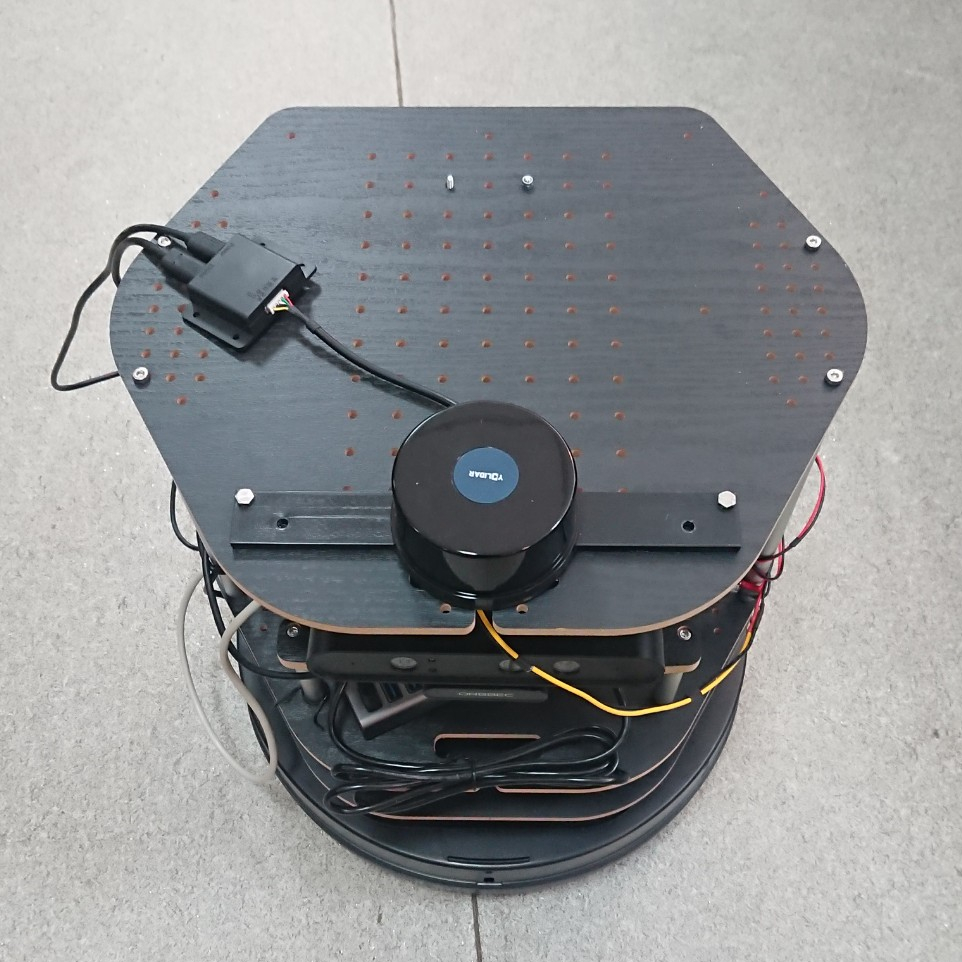
\includegraphics[scale=0.09]{./figures/slides/ch5/tb_yd.jpg}
                \end{figure}
              \end{minipage}
              }
              \hfill
              \noindent\makebox[0.6\linewidth][c]{%
              \scriptsize
              \begin{minipage}{0.6\linewidth}
                \begin{table}[h]\centering \vspace{0.5cm}
                        \begin{tabular}{rc}
                          Απόσταση $d$ [mm]    & Μέσο σφάλμα [mm]   \\ \toprule
                          $50$-$5000$          & $\leq \pm 60$      \\
                          $5000$-$20000$       & $\leq \pm 40$      \\
                          $20000$-$30000$      & $\leq \pm 100$     \\ \bottomrule
                        \end{tabular}
                        \caption{Μέσο σφάλμα μέτρησης αισθητήρα ανά επιστρεφόμενη τιμή απόστασης. Πηγή: datasheet κατασκευαστή}
                \end{table}
              \end{minipage}
    }
    \end{itemize}
  \end{itemize}

\end{frame}
